\chapter{Univariate analysis}
\label{ch:univariate-analysis}

After performing a number of measurements in a sample for a given population, researchers want to investigate the characteristics of the whole group. It is impractical to consider or list all measurements separately. To gain insight into the collected data, techniques are required to visualize and summarize the data. These techniques are called \emph{descriptive statistics}.


\begin{definition}[Descriptive statistics]
  Descriptive statistics\index{statistics!descriptive} are a collection of techniques to quantitatively describe and summarize features of a collection of information.
\end{definition}

The techniques covered in this chapter deal with the analysis of a single variable (= \emph{univariate analysis}). Chapter~\ref{ch:bivariate-analysis} extends this, by introducing techniques for analyzing relationships between two variables.

\section{Learning Goals}
\label{sec:analyse1var-leerdoelen}

By the end of this chapter you must be able to:

\begin{itemize}
    \item Specify the appropriate central tendency and dispersion for each measurement level;
    \item Reproduce and understand the formules for calculating the mean, variance, and standard deviation of a sample;
    \item Calculate the central tendency and dispersion of a given variable;
    \item Identify suitable visualization techniques for each measurement level;
    \item Apply visualization techniques suitable for a given variable;
    \item Interpret a given graph, this includes naming the graph type, and deriving the central tendency and dispersion.
\end{itemize}

\section{Central Tendency and Dispersion}

Imagine a group of researchers want to conduct a study on superheroes. Questions they could ask include:

\begin{itemize}
    \item How tall are superheroes usually?
    \item What is their weight?
    \item How successful are they in making the community safe?
    \item How many people do they rescue?
    \item \ldots
\end{itemize}

To summarize the results of measurements, there are different methods that depend on the measurement level of the variable in question. On the one hand we look for a value that is representative of the entire group, the \index{central tendency}\emph{central tendency}, and on the other hand we are looking for a value that indicates how large the mutual differences are within the group, the \index{dispersion}\emph{dispersion}. The combination of central tendency and dispersion is often used when summarizing a series of measurements.

Table~\ref{tab:centrum-spreidingsmaten} provides an overview of suitable measures for the central tendency and the dispersion. These are defined later in this chapter.


\begin{table}
    \centering
    \begin{tabular}{lll}
        \toprule
        \textbf{Measurement Level}  & \textbf{Central Tendency} & \textbf{Dispersion} \\
        \midrule
        Qualitative                 & mode                      & ---                 \\
        \midrule
        Quantitative                & mean            & variance, standard deviation  \\
                                    & median          & range, interquartile range    \\
        \bottomrule
    \end{tabular}
    \caption[Suitable measures for central tendency and dispersion for each measurement level.]{Suitable measures for central tendency and dispersion for each measurement level. The combination of central tendency and dispersion is often used when summarizing a series of measurements.}
    \label{tab:centrum-spreidingsmaten}
\end{table}

\section{Qualitative Variables}
With qualitative variables, the value is not necessarily a number. For example, a qualitative variable 'gender' has values such as \emph{man} and \emph{woman}. This makes calculations difficult. As a result, possibilities for summarizing the values are limited. We can use the \emph{mode} as central tendency, but there is no real measure for the dispersion. To show the spread over the various occurring values, you could use a frequency table that indicates how often each value occurs in the data set.

\subsection{Mode}

\begin{definition}[Mode]
    The \emph{mode} is the value that appears most often in a dataset.
\end{definition}

\begin{itemize}
    \item There can be two modi, in this case we call the dataset \index{bimodal}\emph{bimodal};
    \item There can even be more than two modes, when the dataset is \index{multimodal} \emph{multimodal}.
    \item The mode does not make much sense when describing a quantitative variable, since each measurement is typically unique. However, in this case it could sometimes be useful to group them into categories (cfr. Example~\ref{ex:modal-class}).
\end{itemize}

\begin{example}
    \label{ex:modal-class}
    Researchers have kept track of how many people Batman rescued each year. 
    Below are the numbers for the last nine years, divided into 4 categories.
    
    \begin{itemize}
        \item $[0-9]$ people : 4, 7
        \item $[10-19]$ people: 11, 16
        \item $[20-29]$ people : 20, 22, 25, 26
        \item $[30-39]$ people: 33
    \end{itemize}
    
    Category $[20-29]$ occurs the most, and is called the \emph{modal class}. We could use the center of this range, i.e.~25, as the mode.
\end{example}

\section{Quantitave Variables}

With quantitative variables, there  are more possibilities for describing the central tendency and dispersion. For these variables, you could for example use:

\begin{itemize}
    \item a mean and standard deviation;
    \item a median and interquartila range.
\end{itemize}

Suppose the researchers carried out a number of measurements regarding the length of superheroes. The results can be found in Figure~\ref{fig:heroes-size}.

\begin{figure}
  \centering
\begin{tikzpicture}[xscale=4,yscale=2]
\draw (0,2) -- (0,0);
\foreach \num/\label in {0/0, 0.2/20, .4/40, .6/60, .8/80, 1/100, 1.2/120, 1.4/140, 1.6/160, 1.8/180, 2/200}{%
    \draw (0, \num) -- (2.5, \num);
    \draw[shift={(0, \num)}] (1pt,0pt) -- (-1pt,0pt) node[left] {\scriptsize \label};
}

\node[anchor=north] (hero1) at (0.3,1.5)
{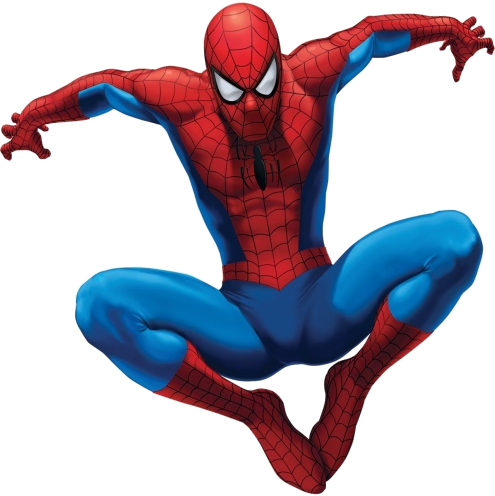
\includegraphics[height=2.9cm]{les2-hero-1}};
\node[anchor=north] (hero2) at (0.8,2.05)
{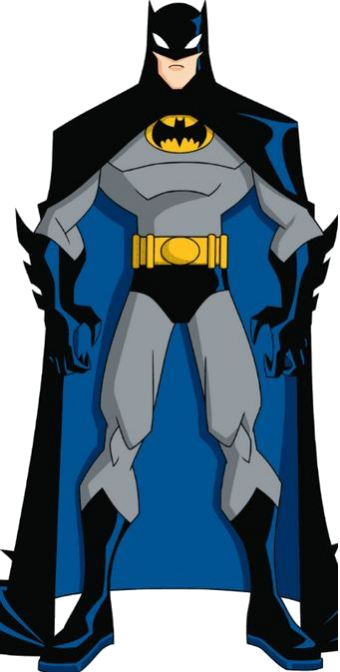
\includegraphics[height=4cm]{les2-hero-2}};
\node[anchor=north] (hero3) at (1.3,1.575)
{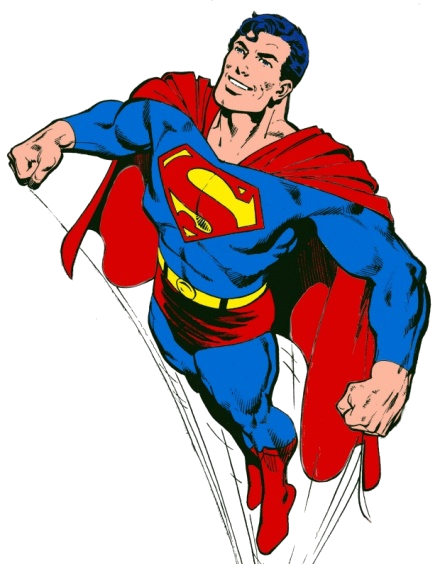
\includegraphics[height=3.1cm]{les2-hero-3}};
\node[anchor=north] (hero4) at (1.8,2.1)
{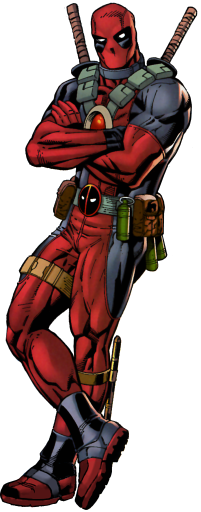
\includegraphics[height=4.1cm]{les2-hero-4}};
\node[anchor=north] (hero5) at (2.3,1.95)
{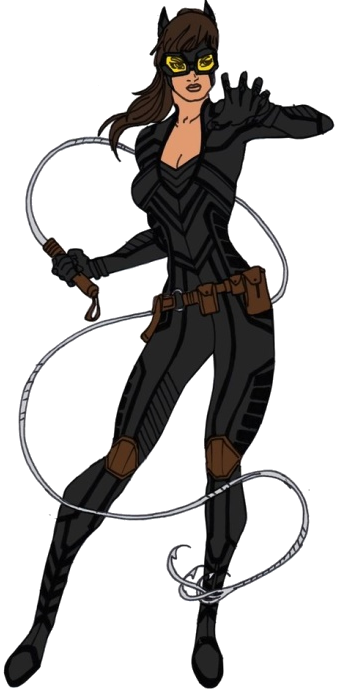
\includegraphics[height=3.8cm]{les2-hero-5}};

\node (size1) at (0.3, 1.5) {\scriptsize 141 cm};
\node (size2) at (0.8, 2.1) {\scriptsize 198 cm};
\node (size3) at (1.3, 1.51) {\scriptsize 143 cm};
\node (size4) at (1.8, 2.15) {\scriptsize 201 cm};
\node (size5) at (2.3, 1.95) {\scriptsize 184 cm};
\end{tikzpicture}

  \caption{Superhero sizes, in cm.}
  \label{fig:heroes-size}
\end{figure}

\subsection{Arithmetic mean}
\label{ssec:arithmetic-mean}

\begin{definition}[Arithmetic mean]
    \label{def:mean}
    
    The \emph{arithmetic mean}\index{mean!arithmetic} or \emph{average} (notation $\overline{x}$, x-bar) of a set of values is the sum of all values divided by the number of values.
    \begin{equation}
    \overline{x} = \frac{1}{n} \times \sum_{i=1}^{n} x_{i}
    \label{eq:Mean}
    \end{equation}
    
    With:
    \begin{itemize}
        \item $x_{i}$ the different values of a set (in the example of Figure~\ref{fig:heroes-size}: 141, 198, 143, etc.)
        \item $n$ the number of values (in the example is $n = 5$).
    \end{itemize}
\end{definition}

\begin{remark}[!!]
    Note that the symbol $\overline{x}$ specifically indicates the average of a \emph{sample}.
    The average of a \emph{population} is indicated by the Greek letter mu, $\mu $.
    
    See Appendix~\ref{app:notation} for an overview of the symbols and notations used in this syllabus.
\end{remark}

\begin{exercise}
    What is the average length of the superheroes in Figure~\ref{fig:heroes-size}?
\end{exercise}

\begin{exercise}
    The average of 15 numbers is 12. What number do we need to add to get an average of 13?
\end{exercise}

\begin{exercise}
    The arithmetic mean is sensitive to outliers, i.e. values far away from the mean. Extreme values can heavily influence the arithmetic mean.
    
    Assume that Kabout Wesley (10 cm) is added to the team of superheroes. What happens to the arithmetic mean?
\end{exercise}

\subsection{Variance and standard deviation}
\label{ssec:variance-and-standard-deviation}

The dispersion measure that is typically associated with the average is the standard deviation.
Before defining the standard deviation, we first provide the definition of the \emph{variance}.

\begin{definition}[Variance]
    The \emph{variance}\index{variance} (notation: $s^{2}$) of a sample is the mean squared difference between the values of the sample and the arithmetic mean.
    \begin{equation}
    s^{2} = \frac{1}{n-1} \times \sum_{i=1}^{n} \left( \overline{x} - x_i \right)^{2}
    \label{eq:variance}
    \end{equation}
\end{definition}

You may have noticed that in the formula the denominator is $n-1$ and not $n$, which you would expect. However, there is a variant of the formula with $n$ in the denominator. This latter one is called the population variance, indicated by $\sigma^2 $ (the Greek letter sigma).

The variance of a sample is used in practice as an estimate for the (unknown) population variance. The formula with $n-1$ in the denominator is a so-called \textit{pure estimator}, which means that in many repetitions the average of the estimates converges to the population variance. You can prove this mathematically, but this is beyond the scope of this course.

\begin{example}
    The variance of the length of our superheroes is calculated as follows:
    
    \begin{align*}
    s^{2} & =  \frac{(173,4 - 141)^{2} + (173,4 - 198 )^{2} + (173,4 - 143)^{2} + (173,4 - 201)^{2} + (173,4 - 184 )^{2}}{4} \\
    & =  \frac{(-32,4)^{2} + (24,6)^{2} + (-30,4)^{2} + (27,6)^{2} + (10,6)^{2}}{4}                                    \\
    & = \frac{1049,76 + 605,16 + 924,16 + 761,76 + 112,36}{4}                                                          \\
    & = \frac{3453,2}{4} = 863,3
    \end{align*}
\end{example}

When calculating the variance of our sample, we divide by $n-1$ and not by $n$. Why? 
As the sum of the deviations $x_{i} - \overline {x} $ always returns 0 (see below in Equation~\ref{eq:sumAvg}), the last deviation can be derived from the first $n-1$ deviations. Therefore we do not calculate the average of $n$ numbers without relationship. Only $n-1$ of the squared deviations can move freely, so we calculate the average by dividing the total by $n-1$. The number $n-1$, the number of logically independent values, is also called the \index{degrees of freedom} \emph{degrees of freedom}.

\begin{equation}
\sum_{i}^{n}(x_{i} - \overline{x}) = \sum_{i}^{n}x_{i} - \sum_{i}^{n}\overline{x} = \sum_{i}^{n}x_{i} - n \left(\frac{1}{n}\sum_{i}^{n} x_{i}\right)
\label{eq:sumAvg}
\end{equation}

\begin{definition}[Standard deviation]
    The \emph{standard deviation}\index{standard deviation} is the square root of the variance.
    \begin{equation}
    s = \sqrt{s^{2}} = \sqrt{\frac{1}{n-1} \sum_{i=1}^{n} \left(\overline{x} - x_i \right)^{2}}
    \label{eq:stdev}
    \end{equation}
\end{definition}

\begin{remark}[!!]
    In this definition we also explicitly defined the variance and standard deviation of a \emph{sample}. The standard deviation of a \emph{population} is indicated by the Greek letter sigma, $\sigma$.
\end{remark}

The standard deviation provides insight into what is normal and abnormal: 
A small standard deviation indicates that the values are close to the central tendency (arithmetic mean, $\overline{x}$),while  a large standard deviation indicates that the values are dispersed over a larger range of values. In some cases, a small standard deviation is desired, in other cases, it may not be that important, as illustrated below.

\begin{example}
  In the manufacturing process of screw drivers, the size of the head is important for its functioning. When the heads of a batch of 1000 screw drivers is measured, their sizes should be very similar, so a very small standard deviation is an indication of good quality.    
\end{example}

\begin{example}
  Super heroes are a very diverse group. Some are very rich (e.g.~Batman, Iron Man), some are middle class (e.g.~Spiderman), others are quite poor (e.g.~Arsenal). The dispersion of their income would be very large, but that isn't necessarily a bad thing.
\end{example}

An interesting property of the standard deviation is that it is expressed in the same unit as the measured data. In the example (size of superheroes), the standard deviation is 29,38 cm. 

Just like the arithmetic mean, the variance and standard deviation are sensitive to outliers. The variance is even more sensitive than the mean, because of the squared differences.

\subsection{Median}
\label{ssec:median}

The median is also a measure for central tendency. Compared to the arithmetic mean, the median is much less sensitive to outliers.

\begin{definition}[Median]
    The \emph{median}\index{median} is the value separating the higher half of a data set from the lower half. When you sort the values from low to high, the median will be the value in the middle. If the set has an even number of values, the median is the average of the two values in the middle. 
\end{definition}

\begin{exercise}
    What is de median of the sizes of our superheroes?
\end{exercise}

\begin{exercise}
    What would be the median if Kabouter Wesley (10 cm) is added to the group? 
    Is the impact bigger or smaller compared to the arithmetic mean?
\end{exercise}

\subsection{Range}
\label{ssec:range}

\begin{definition}[Range]
    The \emph{range}\index{range} of a dataset is the absolute value of the difference between the highest and the lowest value.
    \begin{equation}
    | max_i(x_i) - min_i(x_i) |
    \end{equation}    
\end{definition}

The range of a variable is often not interesting as a measure for dispersion, because it is very sensitive to outliers.


\subsection{Quartiles and Interquartile Range}
\label{ssec:quartiles}

The interquartile range is a better measure for dispersion, as it is less sensitive to outliers.
To understand the interquartile range, we first have to introduce the concept of \emph{quartiles}.

\begin{definition}[Quartiles]
    The \emph{quartiles}\index{quartiles} of a sorted set of numbers are the three values that divide the set into 4 equally large subsets.
    
    \begin{itemize}
        \item the first/lower quartile ($Q_{1}$) is the value that separates the lowest quarter of values from the rest
        \item the second quartile ($Q_{2}$) is the value that separates the lowest half of values from the highest half.
        \item the third/higher quartile ($Q_{3}$) is the value that separates the highest quarter of values from the rest
    \end{itemize}
\end{definition}

To determine the values of the quartiles in a sorted set, you can follow this approach~\autocite{Moore2002}:

If $n$ is an odd number, then:
\begin{itemize}
    \item $Q_{1}$ is the $\frac{n+1}{4}$th value;
    \item $Q_{3}$ is the $\frac{3n+3}{4}$th value.
\end{itemize}

If $n$ is an even number:
\begin{itemize}
    \item $Q_{1}$ is the $\frac{n+2}{4}$th value;
    \item $Q_{3}$ is the $\frac{3n+2}{4}$th value.
\end{itemize}

\begin{exercise}
    The second quartile, $Q_2$ corresponds to which other metric introduced in this chapter?
\end{exercise}

\begin{definition}[Interquartile range]
    The \emph{interquartile range}\index{range!interquartile} ($IQR$) is the difference between the higher and lower quartile.
    \begin{equation}
    IQR = Q_3 - Q_1
    \end{equation}
\end{definition}

The concept of quartiles can be generalized to percentages. The $P$-th \emph{percentile} of a list of ordered values is the smallest value in the list so that $P$ percent of the data is less than or equal to that value.


\section{Visualization of a Single Variable}

Even when visualizing one variable, the most suitable chart type depends on the measurement level.
Table~\ref{tab:charttypes-1-variable} provides an overview.
.

\begin{table}
    \centering
    \begin{tabular}{ll}
        \toprule
        \textbf{Measurement Level} & \textbf{Chart Type}   \\
        \midrule
        Qualitative         & Bar chart of frequencies     \\
        \midrule
        Quantitative        & Box plot, histogram, density \\
        \bottomrule
    \end{tabular}
    \caption{Suitable chart types per measurement level for visualizing a single variable.}
    \label{tab:charttypes-1-variable}
\end{table}

\subsection{Bar Chart}

When visualizing a qualitative variable, a frequency table is first calculated for all occurring values.

\begin{definition}[Frequency table]
    A \emph{frequency table}\index{frequency table} is a table that summerizes how often each value occurs in the data set.
    Frequency tables are usually vertically oriented.
\end{definition}

To draw a \index{bar chart}\emph{bar chart} (cfr. Figure~\ref{fig:barchart}), the different values are listed below the X-axis and for each value a bar is drawn whose height is determined by the number of times the corresponding value occurs.

\begin{figure}
    \centering
    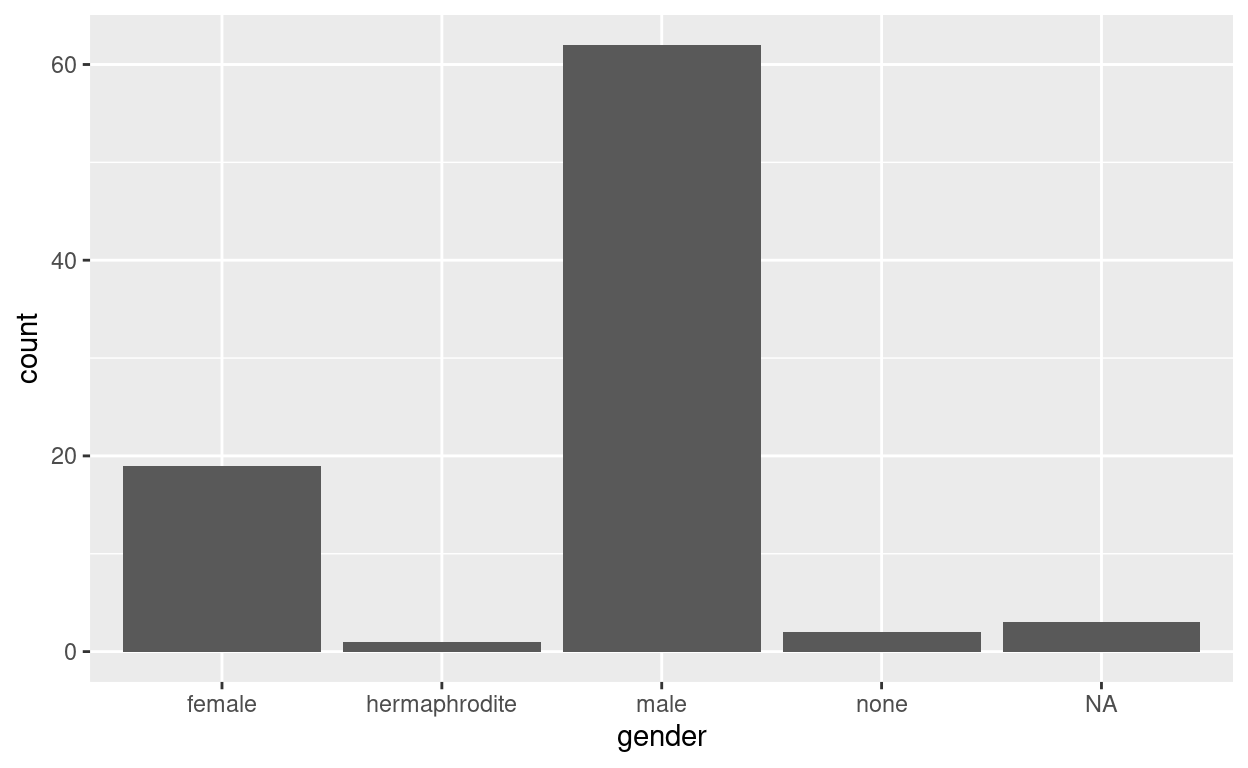
\includegraphics[width=.7\textwidth]{barchart}
    \caption[Example of a bar chart]{\textbf{Example of a bar chart.} The labels on the x-axis indicate the possible values of the visualized qualitative variable. The height of each bar indicates the frequency of each value within the sample.}
    \label{fig:barchart}
\end{figure}

\subsection{Box Plot}

A \index{box plot}\emph{box plot} is a chart that shows the dispersion of a set of values (cfr. Figure~\ref{fig:boxplot}). It is formed by a rectangle with sides at the quartiles ($Q_1$ and $Q_3$). Inside the rectangle, the median is drawn as well. The whiskers attached to the upper and lower sides of the rectangle cover the rest of the observations, except for outliers and extremes.

\begin{itemize}
    \item An \emph{outlier}\index{outlier} is a value that is more than 1.5 times the IQR below the lower quartile or above the higher quartile. It is indicated by a circle.
    \item An \emph{extreme value}\index{extreme} is a value that is more than 3 times the IQR below the lower quartile or above the higher quartile. It is indicated by a star.
\end{itemize}

A box plot is oriented horizontally or vertically, based on what is clearest.

\begin{figure}
    \centering
    % Source: http://mirrors.ibiblio.org/CTAN/graphics/pgf/contrib/pgfplots/doc/pgfplots.pdf
    % p.430
    \begin{tikzpicture}
    \begin{axis}[x=3cm,xticklabels={},xmax=2.3]
    \addplot+[
    boxplot prepared={
        draw direction=y,
        lower whisker=5,
        lower quartile=7,
        median=8.5,
        upper quartile=9.5,
        upper whisker=10,
    },
    ]
    table[row sep=\\,y index=0] {
        data\\ 1\\ 3\\
    }
    [right,color=hgorange]
    node at (boxplot box cs: 1,.6) {outlier}
    node at (boxplot box cs: \boxplotvalue{lower quartile},1) {$Q_1$}
    node at (boxplot box cs: \boxplotvalue{median},1)         {$Q_2$, median}
    node at (boxplot box cs: \boxplotvalue{upper quartile},1) {$Q_3$}
    node at (boxplot box cs: \boxplotvalue{upper whisker},1)  {max}
    ;
    \end{axis}
    \end{tikzpicture}
    \caption[Example of a box plot]{\textbf{Example of a box plot.} The blue rectangle indicates the interval in which half of the measured values are located. The limits are the first quartile at the bottom ($Q_1$) and the third quartile at the top ($Q_3$). The line in the middle of the rectangle is the median (or the second quartile, $Q_2$). The other blue horizontal lines in theory indicate the smallest and largest values. In this case, however, there are some observations that are very far from the median. These are called outliers and are plotted separately as individual points.}
    \label{fig:boxplot}
\end{figure}

\subsection{Histogram}

A \index{histogram}\emph{histogram} (cfr. Figure~\ref{fig:histogram}) is a kind of bar chart, but adjusted for quantitative variables.
The range of the variable is subdivided into a number of, typically equal, intervals or classes. For each class, the number of observations is counted and the height of the bars is determined based on this number.

\begin{figure}
    \centering
    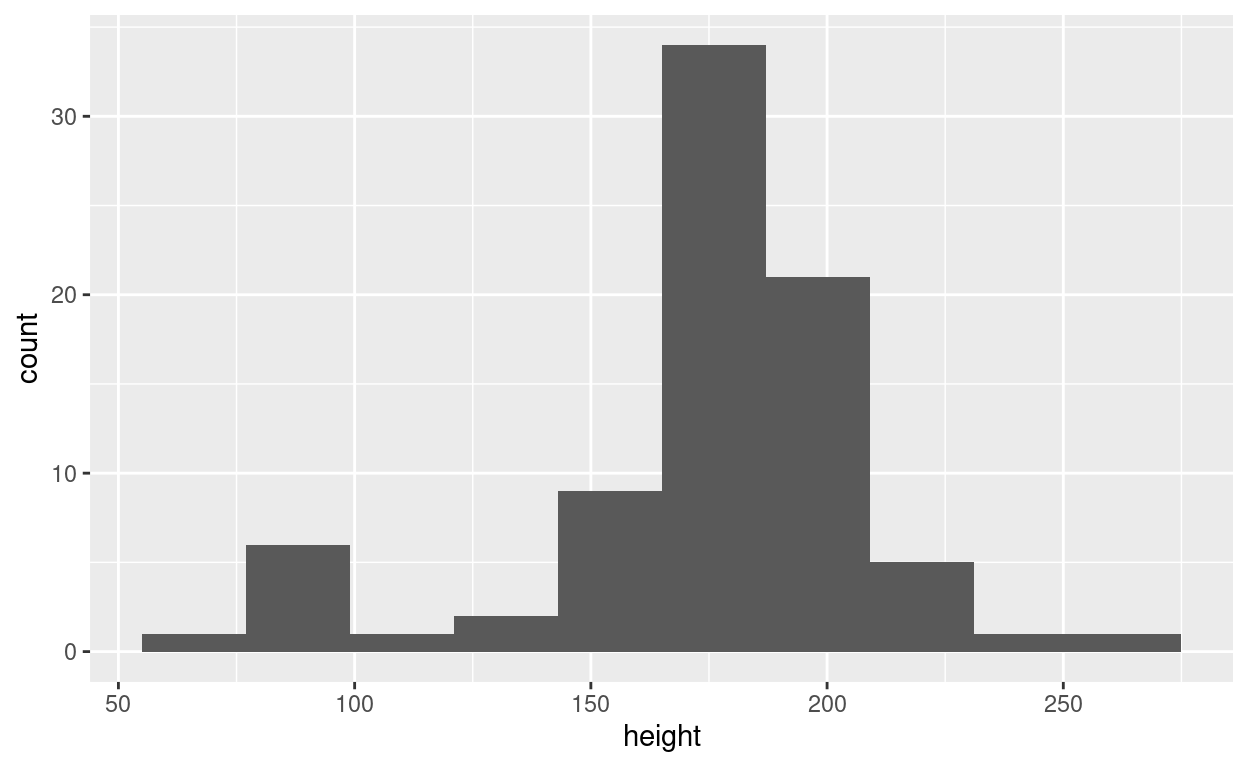
\includegraphics[width=.7\textwidth]{histogram}
    \caption[Example of a histogram]{\textbf{Example of a histogram.} The X-axis is subdivided into a number of equally large intervals. The height of each bar is based on the number of observations within each interval.}
    \label{fig:histogram}
\end{figure}

\subsection{Density Graph}

The clarity of a histogram largely depends on the choice of intervals. If these are chosen too large, you will lose precision, and if they are too small, different intervals will not contain any observations. As an alternative to a histogram, you can also plot a \index{density graph}\emph{density graph} (cfr. Figure~\ref{fig:dichtheidsgrafiek}). In this graph, the X-axis is not subdivided into classes. Instead, a continuous curve is drawn, and the height of this curve corresponds to the amount of observations ``in the neighborhood''. A density graph typically shows even better how the observations are spread.

\begin{figure}
    \centering
    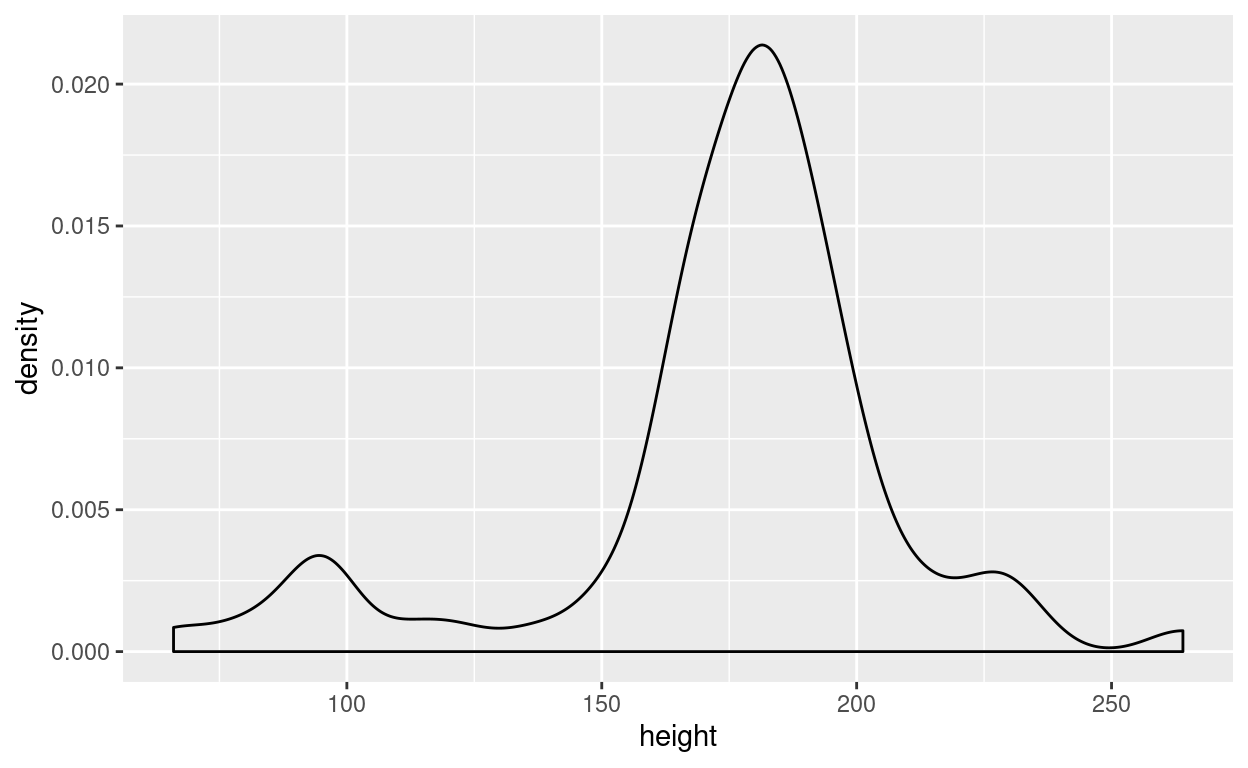
\includegraphics[width=.7\textwidth]{dichtheidsgrafiek}
    \caption[Example of a density graph]{\textbf{Example of a density graph.} The graph shows the same data as the histogram in Figure~\ref{fig:histogram}.}
    \label{fig:dichtheidsgrafiek}
\end{figure}

\section{Exercises}
\label{sec:exercises-univariate-analysis}

\subsection{Central Tendency and Dispersion}

\begin{exercise}
  \label{ex:mean-stdev-freq}
  The formulas for the sample mean $\overline{x}$, variance $s^2$ and standard deviation $s$ can be found in Section~\ref{ssec:arithmetic-mean} and~\ref{ssec:variance-and-standard-deviation} respectively.
  How should these formulas  be adapted to be used with a frequency table? Apply these formulas to the data provided in Table~\ref{tab:pinfreq}.
\end{exercise}

\begin{table}
  \centering
  \begin{tabular}{@{}ll@{}}
    \toprule
    Pins $x$ & Frequency $f_{x}$ \\ 
    \midrule
        0      &         2          \\
        1      &         1          \\
        2      &         2          \\
        3      &         0          \\
        4      &         2          \\
        5      &         4          \\
        6      &         9          \\
        7      &         11         \\
        8      &         13         \\
        9      &         8          \\
        10     &         8          \\
    \bottomrule
  \end{tabular}
  \caption{Frequency table for the number of pins knocked down in a game of bowling.}
  \label{tab:pinfreq}
\end{table}

\begin{exercise}
  \label{ex:variance-formula}
  Why does variance (see Equation~\ref{eq:variance}) use the square of the differences? Why not the actual values themselves (i.e. $(\overline{x} - x_i)$) or the absolute value of the difference (i.e. $\left|\overline{x} - x_i\right|$)?
  
  \begin{align}
  s^{2}_{1} &= \frac{1}{n-1} \sum_{i=1}^{n} (\overline{x} - x) \\
  s^{2}_{2} &= \frac{1}{n-1} \sum_{i=1}^{n} \left| \overline{x} - x\right| \\
  s^{2}_{3} &= \frac{1}{n-1} \sum_{i=1}^{n} (\overline{x} - x)^{2}
  \end{align}
  
  Try out each variant of the equation for both datasets $X = \left\{4,4,-4,-4\right\}$ and $Y = \left\{7,1,-6,-2\right\}$.
\end{exercise}

\begin{exercise}
  Find out what the \emph{coefficient of variation} (CV) means. How is it defined? What is the major difference with the standard deviation?
\end{exercise}

\begin{exercise}
  \label{ex:ais}
  Import the file \texttt{ais.csv} in R (this file is available in the Github repository of this course, inside the folder \texttt{exercises/datasets}). 
  A description of this data frame can be found in the same folder, file \texttt{ais.html}.

  You can import this file in R using the following code:
  \begin{lstlisting}
  ais <- read.csv("ais.csv", sep = ",")
  attach(ais)
  \end{lstlisting}

  Consider the following subsets of this data frame, and calculate for each subset the appropriate measures for central tendency and dispersion for the variables \texttt{sex} and \texttt{ht}.

  \begin{enumerate}
      \item the rowers;
      \item the rowers, the netballers and the tennis players combined;
      \item the female basketball players and rowers.
  \end{enumerate}
\end{exercise}

\begin{exercise}
  \label{ex:mean-range-R}
  Use the functions \texttt{mean} and \texttt{range} in R to determine the mean and range of:
  \begin{itemize}
      \item the numbers 1, 2, \dots, 21.
      \item 50 random values, generated from a normal distribution with mean 0 and variance 1 (function \texttt{rnorm}).
      \item the columns \texttt{height} and \texttt{weight} of the data frame \texttt{women} (built-in in R).
  \end{itemize}
\end{exercise}


In previous exercises we described the different measures for central tendency and dispersion.
As you might have notices, these metrics are also used in the research of~\textcite{Akin2016}.
In the next exercies, we will try to reproduce the results.

For this, we need the file \texttt{android\_persistence\_cpu.csv}.
This file can also be found inside the folder \texttt{exercises/datasets} on GitHub.


\begin{exercise}
  \label{oef:casus-akin2016-1var}
  Open this file in a spreadsheet application and study the structure of the data. 
  Can you identify the variables and their measurement level?
\end{exercise}

We will be using the \texttt{R} programming language for statistical computing with RStudio. 

\begin{lstlisting}[breaklines=true]
  android_cpu <- read.csv("android_persistence_cpu.csv", sep=";", dec=".")
  attach(android_cpu)
\end{lstlisting}

You can use the above code to import the file in R. 
After importing the file, try to calculate the average execution time, the standard deviation, the different quantiles, etc.
Use the commands \texttt{mean}, \texttt {median}, \texttt {quantile}, \texttt {min}, \texttt{max}, \texttt{var}, \texttt{sd}. 
You can also use the \texttt{summary} command to get a nice overviw.

Tips:

\begin{itemize}
  \item A column/variable of a data table is referred to as: \verb|Table$Column|. When you have \verb|attach|ed the table, you can use the \verb|Column| name directly.
  \item You can group values according to a qualitative value with \verb|Variable ~ Categories|.
\end{itemize}


\begin{exercise}
  Is it possible to draw conclusions from these results? If so, what are they? If not, why not?
\end{exercise}

\subsection{Charts in R}
\subsubsection{Histogram}

A histogram is a plot that shows the frequencies of observations between specific ranges.

\begin{lstlisting}[breaklines=true]
  hist(android_cpu$Time, main="Distribution of execution time", xlab="Execution time (ms)")
  hist(android_cpu$Time, main="Distribution of execution time", xlab="Execution time (ms)", breaks=2)
\end{lstlisting}

\begin{exercise}
  Can you draw useful conclusions from this graph\footnote{You can find general info about generating plots in R here:  \url{https://www.datacamp.com/community/tutorials/15-questions-about-r-plots\#gs.RK_ORsI}.}? 
  What happens if you increase the number of \texttt{breaks}?
\end{exercise}

\subsubsection{Boxplot}

A boxplot shows the median, quartiles, and extremes in a dataset. 
It provides a good overview of the distribution of the data.

\begin{lstlisting}[breaklines=true]
  boxplot(android_cpu$Time)
  boxplot(android_cpu$Time, main='Distribution of execution time', ylab="Execution time (ms)")
\end{lstlisting} 

\begin{exercise}
  By default, boxplots are drawn vertically. Use the help function in RStudio to find out how to draw it horizontally.
\end{exercise}

In the previous exercises, when we tried to analyse the dataset as a whole, we noticed that this is pretty much useless, since the data set is divided into several categories. 
Let's create separate boxplots for each category.

\begin{lstlisting}[breaklines=true]
  boxplot(android_cpu$Time ~ android_cpu$DataSize, main="Distribution of CPU time over the data sizes", ylab="Time in ms");
\end{lstlisting}

\begin{exercise}
	\label{ex:boxplot}
  Interpret the results from this plot. Do these make more sense?
\end{exercise}

We can do the same for the different persistence types.

\begin{exercise}
  Do the same as in \ref{ex:boxplot}, but group by \verb|PersistenceType| and interpret the results. Do these make sense?
\end{exercise}

Finally, let's see how the data is distributed over \emph{both} categories.

\begin{lstlisting}[breaklines=true]
  boxplot(android_cpu$Time ~ android_cpu$PersistenceType * android_cpu$DataSize, main="Distribution of CPU time over data sizes for the different persistent types", ylab="Time in ms");
\end{lstlisting}

By looking at the data over the different categories, we get a clearer view on the data, but the graph is a bit overcrowded now.

There are several ways of selecting data that meets specific criteria, a.o.~the functions \verb|which| and \verb|subset|.

\begin{lstlisting}[breaklines=true]
  greenDOA <- android_cpu[which(android_cpu$PersistenceType=='GreenDAO'),];
  boxplot(greenDOA$Time ~ greenDOA$DataSize);
\end{lstlisting}

\begin{exercise}
  Wat can you conclude from this plot?
\end{exercise}

\begin{exercise}
  Find out which box plots are meaningful for this data and whether your results match those of~\textcite{Akin2016}. What are your conclusions?
\end{exercise}

\begin{exercise}[Retrieval practice]
  Use the procedure for retrieval practice from exercise~\ref{ex:retrieval-practice-meetniveaus} 
  to study the \emph{techqniques for analysis and visualization of a single variable}.
  
  Provide for each measurement level:
  
  \begin{itemize}
    \item The appropriate measurements for central tendency and dispersion (name + definitions and formulas)
    \item The appropriate graph types
  \end{itemize}
\end{exercise}




%Exercise~\ref{ex:q2}: the median

%Exercise~\ref{ex:variance-formula}:

%\begin{itemize}
  %\item When using the values themselves, negative and positive values would cancel out each other, resulting in a variance of 0 in set $X$.
  %\item When using the absolute value, both data sets would have the same variance, although the dispersion of set $Y$ is clearly larger.
%  \item When squaring the differences, these problems do not occur.
%\end{itemize}



% Answers
\section{Solutions to selected exercises}

\paragraph{Exercise \ref{ex:mean-stdev-freq}}

\begin{itemize}
  \item $\overline{x} = 7$
  \item $s^2 \approx 5.830508$
  \item $s \approx 2.414645$
\end{itemize}

\paragraph{Exercise \ref{ex:variance-formula}}
Table~\ref{tab:opl-variance-ht} provides an overview of the adjusted sample variance for both datasets.

\begin{table}
  \centering
  \begin{tabular}{@{}l|rrr@{}}
    \toprule
      & \textbf{$s^{2}_{1}$} & \textbf{$s^{2}_{2}$} & \textbf{$s^{2}_{3}$} \\
    \midrule                
      \textbf{$ X $} & 0           & 5.333333    & 21.33333    \\ 
      \textbf{$ Y $} & 0           & 5.333333    & 30          \\           
    \bottomrule
  \end{tabular}
  \caption{Results of the adjusted sample variance for both datasets, for the different formulas of exercise~\ref{ex:variance-formula}.}
  \label{tab:opl-variance-ht}
\end{table}

\paragraph{Exercise \ref{ex:ais}}

Table~\ref{tab:opl-ais-ht} provides an overview of the most important measurements for central tendency and dispersion for the variable \texttt{ht} (height/length) for the requested groups.

\begin{table}
  \centering
  \begin{tabular}{@{}l|r|rrrr|rr@{}}
    \toprule
    & \textbf{(1)} & \multicolumn{4}{c}{\textbf{(2)}}                                                 & \multicolumn{2}{c}{\textbf{(3)}} \\ 
    & \textbf{Row} & \textbf{Total}    & \textbf{Row} & \textbf{Netball} & \textbf{Tennis} & \textbf{B\_ball}  & \textbf{Row} \\ \midrule
    \textbf{mean}       & 182.376      & 179.066                      & 182.376      & 176.087          & 174.164         & 182.269           & 178.859      \\
    \textbf{stdev}      & 7.798        & 7.936                        & 7.798        & 4.124            & 9.858           & 8.621             & 5.970        \\
    \textbf{min}        & 156.000      & 156.000                      & 156.000      & 168.600          & 157.900         & 169.100           & 156.000      \\
    \textbf{Q1}         & 179.300      & 174.200                      & 179.300      & 173.450          & 167.300         & 174.000           & 177.600      \\
    \textbf{median}     & 181.800      & 179.500                      & 181.800      & 176.000          & 175.000         & 184.600           & 179.650      \\
    \textbf{Q3}         & 186.300      & 183.400                      & 186.300      & 179.150          & 180.750         & 188.700           & 181.200      \\
    \textbf{max}        & 198.000      & 198.000                      & 198.000      & 183.300          & 190.800         & 195.900           & 186.300      \\
    \textbf{IQR}        & 7.000        & 9.150                        & 7.000        & 5.700            & 13.450          & 14.700            & 3.600        \\ \bottomrule
  \end{tabular}
  \caption{Overview results Exercise~\ref{ex:ais} for the variable \texttt{ht} (height/length).}
  \label{tab:opl-ais-ht}
\end{table}

In part 1 and 2 we take the variable \texttt{sex} as an example, cfr. Table~\ref{tab:opl-ais-sex} for an overview.
We cannot say much about qualitative variables, so we provide a frequency table from which we can derive the mode.

In part 3 only women are selected, and Table~ \ref{tab:opl-ais-sport} illustrates the frequencies of the variable \texttt{sport}.

\begin{table}
  \centering
  \begin{tabular}{@{}l|r|rrrr}
  	\toprule
  	               & \textbf{(1)} &                    \multicolumn{4}{c}{\textbf{(2)}}                     \\
  	               & \textbf{Row} & \textbf{Whole group}& \textbf{Row} & \textbf{Netball} & \textbf{Tennis} \\ \midrule
  	\textbf{f}     &           22 &                  52 &           22 &               23 &               7 \\
  	\textbf{m}     &           15 &                  19 &           15 &                0 &               4 \\
  	\textbf{mode}  &            f &                   f &            f &                f &               f \\ \bottomrule
  \end{tabular}
  \caption{Overview results Exercise~\ref{ex:ais} (1) and (2) for the variable \texttt{sex}. This table provides the different frequencies, as well as the mode.}
  \label{tab:opl-ais-sex}
\end{table}

\begin{table}
  \centering
  \begin{tabular}{@{}l|l}
  	\toprule
  	                 & Frequency   \\ \midrule
  	\textbf{B\_ball} & 13          \\
  	\textbf{Row}     & 22          \\
  	\textbf{modus}   & Row         \\ \bottomrule
  \end{tabular}
  \caption{Overview results Exercise~\ref{ex:ais} (3) for the variable \texttt{sport}.}
  \label{tab:opl-ais-sport}
\end{table}


\paragraph{Exercise \ref{ex:mean-range-R}}
Table~\ref{tab:opl-mean-range-R} provides an overview of the mean and range for exercise~\ref{ex:mean-range-R}.

\begin{table}
  \centering
  \begin{tabular}{@{}l|r|rl@{}}
    \toprule
      & \textbf{Mean} & \multicolumn{2}{c}{\textbf{Range}} \\
    \midrule                
                  \textbf{$1,2,...,21$} & 11       & 1    & 21    \\ 
        \textbf{\texttt{women\$height}} & 65       & 58   & 72    \\
        \textbf{\texttt{women\$weight}} & 136.7333 & 115  & 164   \\
    \bottomrule
  \end{tabular}
  \caption{Mean and range for the datasets of Exercise~\ref{ex:mean-range-R}.}
  \label{tab:opl-mean-range-R}
\end{table}